\chapter{Clustering}
In questo capitolo mostreremo il comportamento 
degli algoritmi di clustering KMeans, DBSCAN 
e Hierarchical applicati al nostro insieme di 
dati.

Il dataset utile per questa fase \`e stato
ottenuto eliminando gli attributi categorici
\texttt{education, sex} e \texttt{status} 
e l'attributo \texttt{credit\_default} 
poich\`e il clustering rientra tra 
gli addestramenti di tipo non supervisionato.

\section{KMeans}

Il miglior parametro \textit{k} con cui eseguire 
KMeans \`e stato stimato calcolando la 
\textit{SSE} variando \textit{k} su un range da 
2 a 20, con metrica di distanza euclidea. 
In figura~\ref{fig:best_k} sono riportati 
i risultati ottenuti. Si nota che il cambio di
pendenza della curva si trova quando \textit{k}
vale 7. A partire da ci\`o abbiamo eseguito l'algoritmo
per $k\in[3,10]$, reiterando per ogni passo 50 volte
KMeans per evitare che la scelta casuale dei centroidi
influenzasse i risultati e calcolando in questo caso
anche l'indice di Silhouette per i cluster trovati.
In seguito a queste analisi abbiamo constatato come
i cluster ottenuti per $k=4$ siano i pi\`u significativi,
la nostra considerazione \`e stata rafforzata dal fatto
che il clustering ottenuto per $k=4$ presenta il valore
dell'indice di \sil pi\`u alto trovato.

\begin{figure}[H]
	\centering
	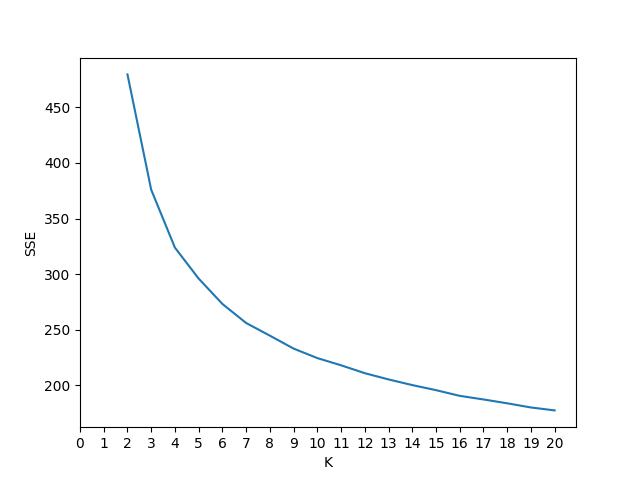
\includegraphics[width=\linewidth]{img/best_k.png}
	\caption[LOF entry]{SSE}
	\label{fig:best_k}
\end{figure} 

Di seguito analizziamo i cluster trovati, assegnando loro 
un nome che contraddistingua le caratteristiche 
di ogni cluster.

\paragraph{Senza rischio}
Cluster costituito da 3032 persone. Pagano in modo puntuale
le loro spese ogni mese senza registrare ritardi e compiono 
solitamente spese di bassa entit\`a. Non costituiscono alcuna
minaccia per la banca.

\paragraph{Piccoli pagatori}
Gruppo di 4832 persone. Sono soliti fare un uso abbastanza 
intensivo del revolving credit per pagare le loro spese. 
Anch'essi registrano spese di bassa entit\`a e non commettono
gravi ritardi nel pagamento, per questo motivo rientrano tra
clienti credibili per la banca.

\paragraph{Grandi pagatori}
Cluster di 1083 persone. Come per i \textit{piccoli pagatori}, 
anch'essi sono soliti usare la modalit\`a di pagamento 
rateizzata anche se le loro spese sono generalmente molto elevate.
Non si registrano comunque grossi ritardi ed \'e per questo che
rientrano comunque tra il gruppo di clienti credibili.

\paragraph{Ritardatari}
Gruppo formato da 1053 persone. Registrano spese di media entit\`a
ma al contrario degli altri tre gruppi si verificano gravi ritardi
nei pagamenti. Sono il cluster di persone che, infine, finisce in
credit default e non sono clienti credibili per la banca.

In figura~\ref{fig:centers} si sono plottate una selezione
delle coordinate dei centroidi, mostrando chiaramente dove i quattro
cluster trovati differiscono maggiormente.

\begin{figure}[H]
	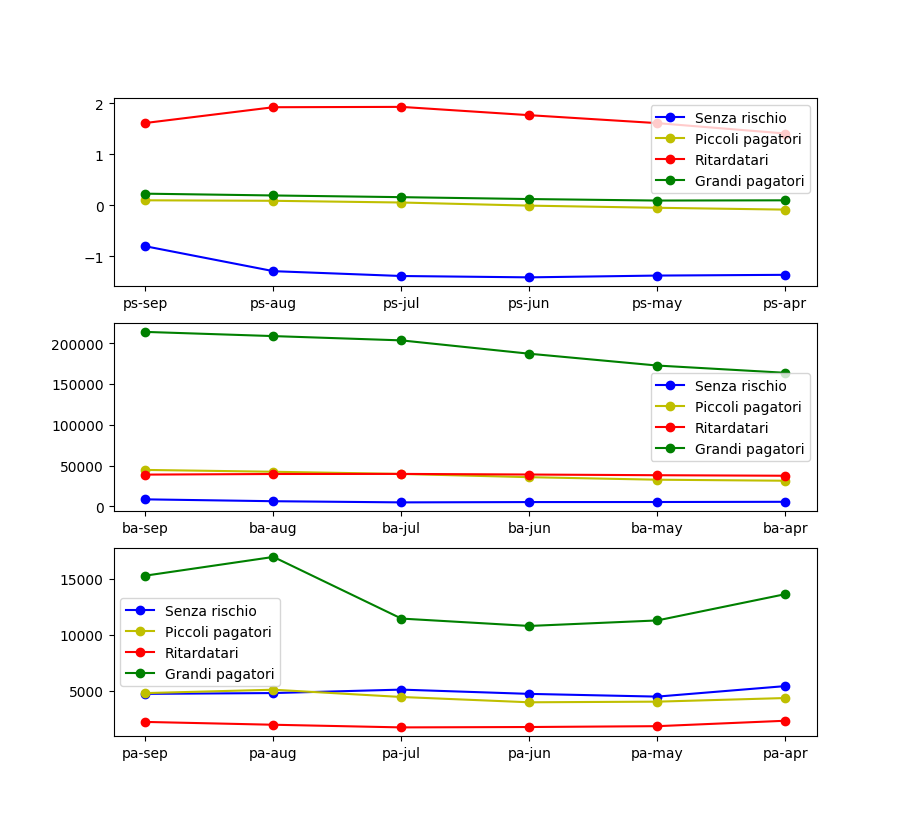
\includegraphics[width=\linewidth]{img/centers_kmeans.png}
	\caption{Caratteristiche dei cluster}
	\label{fig:centers}
\end{figure} 

\begin{figure}[H]
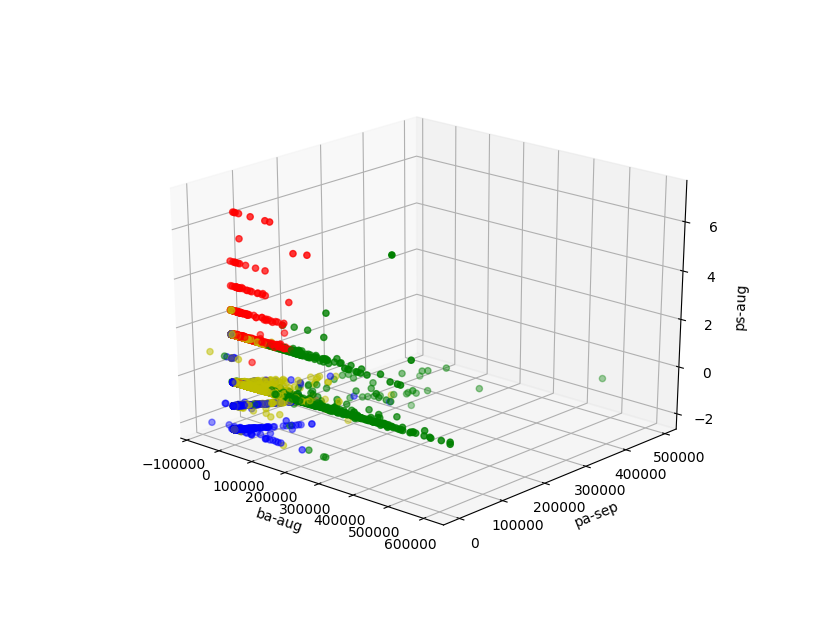
\includegraphics[width=\linewidth]{img/kmeans.png}
\caption{Distribuzione dei cluster su un pagamento mensile}
\label{fig:kmeans}
\end{figure} 

Infine si \`e plottato su un un grafico 3D (figura~\ref{fig:kmeans}
la distribuzione dei cluster su un pagamento mensile (in questo 
caso si e' preso il pagamento del mese di agosto) ed abbiamo 
notato che la distribuzione \`e rispettata per ogni terna di attributi
validi costruibili sull'insieme dei mesi disponibili.
In particolare il cluster dei \textit{ritardari} si posiziona sempre a valori molto elevati di \texttt{payment status}, mentre vale
esattamente il contrario per il cluster dei \textit{senza rischio}.
Le tre
dimensioni scelte per l'esempio sono \texttt{billing amount august},
\texttt{payment status august} e \texttt{payment amount september}.

Infine riportiamo una tabella contenente la media e la deviazione 
standard di ogni cluster individuato. Per ragioni di spazio per 
gli attributi \texttt{payment status}, \texttt{payment amount}
e \texttt{billing amount} mostriamo i valori degli ultimi due mesi.

\begin{center}
	
\begin{tabular}{c|c|c|c|c|c|c}
	\hline
	\textbf{Cluster} & \textbf{ps-sep} 
	& \textbf{ps-aug} & \textbf{pa-sep} 
	& \textbf{pa-aug}\\
	\hline
	Senza rischio & 
	$-0.8 (\pm 1.0)$ & 
	$-1.3 (\pm 0.7)$ &
	$4.7k (\pm 12.0k)$ &
	$4.8k (\pm 14.3)$\\
	\hline
	Piccoli pagatori & 
	$0.09 (\pm 0.71)$ & 
	$0.08 (\pm 0.71)$ &
	$4.8k (\pm 10k)$ &
	$5k (\pm 13.3k)$\\
	\hline
	Grandi pagatori & 
	$0.22 (\pm 0.75)$ & 
	$0.19 (\pm 0.71)$ &
	$15k (\pm 35k)$ &
	$16k (\pm 56k)$\\
	\hline
	Ritardatari & 
	$1.60 (\pm 1.18)$ & 
	$1.90 (\pm 1.03)$ &
	$2k (\pm 3.4k)$ &
	$1.8k (\pm 3.0k)$\\
	\hline
	& 
	\textbf{ba-sep} & 
	\textbf{ba-aug} & 
	\textbf{limit} & 
	\textbf{age} &\\
	\hline
	Senza rischio & 
	$8.7k (\pm 21k)$ &
	$6.4k (\pm 16k)$ &
	$215k (\pm 126k)$ &
	$36 (\pm 8)$\\
	\hline
	Piccoli pagatori &
	$44k (\pm 39k)$ &
	$42k (\pm 35k)$ &
	$130k (\pm 113k)$ &
	$35 (\pm 9)$\\
	\hline
	Grandi pagatori &
	$213k (\pm 93k)$ &
	$208k (\pm 88k)$ &
	$281k (\pm 115k)$ &
	$37 (\pm 8)$\\
	\hline
	Ritardatari &
	$38k (\pm 35k)$ &
	$39k (\pm 36k)$ &
	$79k (\pm 68k)$ &
	$34 (\pm 8)$\\
	\hline
	& 
	\textbf{sex} & 
	\textbf{status} & 
	\textbf{education} & 
	\textbf{default}\\
	\hline
	Senza rischio & 
	F &
	Single &
	University&
	17\%\\
	\hline
	Piccoli pagatori & 
	F &
	Single &
	University&
	18\%\\
	\hline
	Grandi pagatori & 
	F &
	Single &
	University&
	19\%\\
	\hline
	Ritardatari & 
	F &
	Single &
	University&
	61\%\\
	\hline
\end{tabular}

\end{center}

Si noti come il gruppo dei ritardatari ha un limite imposto dalla banca molto pi\`u basso rispetto agli altri cluster. Segno che la banca ha valutato ottimamente i profili nella scelta di concessione del credito.
